\documentclass[a4paper,12pt]{article}
\usepackage{amssymb} % needed for math
\usepackage{amsmath} % needed for math
\usepackage[utf8]{inputenc} % this is needed for german umlauts
\usepackage[ngerman]{babel} % this is needed for german umlauts
\usepackage[T1]{fontenc}    % this is needed for correct output of umlauts in pdf
\usepackage[margin=2.5cm]{geometry} %layout
\usepackage{booktabs}
\usepackage[hidelinks]{hyperref}
\hypersetup{pdftitle={Balanced Banana},bookmarks=true,}
\usepackage{graphicx}
\usepackage{csquotes}
\usepackage[nonumberlist]{glossaries}
\usepackage{enumitem}
\usepackage{verbatim}
\usepackage{indentfirst} % Adds indent for the first paragraph after a {/section}
\usepackage{url}
\newcommand\purl[1]{\protect\url{#1}}



\deftranslation[to=ngerman]{Glossary}{\section{Stichwortverzeichnis}}

\makeatletter
\newenvironment{mycode}
 {\def\@xobeysp{\ }\verbatim\rightskip=0pt plus 6em\relax}
 {\endverbatim}
\makeatother

\setitemize{align=parleft, labelsep=0.5cm}


\makenoidxglossaries



\title{Balanced Banana}
\author{Niklas Lorenz \and Thomas Häuselmann \and Rakan Zeid Al Masri \and Christopher Lukas Homberger \and Jonas Seiler}


%%%%%%%%%%%%%%%%%%%%%%%%%%%%%%%%%%%%%%%%%%%%%%%%%%%%%%%%%%%%%%%%%%%%%%
% Create a shorter version for tables. DO NOT CHANGE               	 %
%%%%%%%%%%%%%%%%%%%%%%%%%%%%%%%%%%%%%%%%%%%%%%%%%%%%%%%%%%%%%%%%%%%%%%
\newcommand\addrow[2]{#1 &#2\\ }

\newcommand\addheading[2]{#1 &#2\\ \hline}
\newcommand\tabularhead{\begin{tabular}{lp{13cm}}
\hline
	}

\newcommand\addmulrow[2]{ \begin{minipage}[t][][t]{2.5cm}#1\end{minipage}%
   &\begin{minipage}[t][][t]{8cm}
    \begin{enumerate} #2   \end{enumerate}
    \end{minipage}\\ }

\newenvironment{usecase}{\tabularhead}
{\hline\end{tabular}}

\usepackage{microtype}

\begin{document}
\pagenumbering{roman}
\begin{titlepage}
    \begin{center}
    
     \vspace*{0.8cm}
 
        
\includegraphics[width=0.5\textwidth]{balancedbanana}
        \vspace*{1cm}
 
        \Huge
        \textbf{Balanced Banana}
 
        \vspace{0.5cm}
        \LARGE
        A Distributed Task Scheduling System
        
        \vspace{0.5 cm}
        \LARGE
        Pflichtenheft
 
        \vspace{1.5cm}

        \large
        \textbf{Niklas Lorenz, Thomas Häuselmann, Rakan Zeid Al Masri, Christopher Lukas Homberger und Jonas Seiler}
 
        \vspace*{0.5cm}

        \textbf{\today}
 
       
        
 
    \end{center}
\end{titlepage}         % Deckblatt.tex laden und einfügen
\setcounter{page}{2}
\tableofcontents          % Inhaltsverzeichnis ausgeben
\clearpage
\pagenumbering{arabic}

% Document starts here.
\section{Einleitung}
\vspace{1cm}

% Here

\clearpage
\section{Aufbau}

\subsection{Architektur}
% Hier soll die verschiedenen Teile unseres Programms erklärt werden.

\subsubsection{Datenbank}

	Die Datenbank enthält relevante Daten über verschiedene Entitäten in unserem Programm. Mit Hilfe von SQL-Queries kann unser Programm diese Daten abrufen und sinnvoll nutzen.  Unsere Datenbank verwendet ein relationales Datenbank-Managementsystem, um Informationen in verschiedenen Tabellen zu speichern. Darüber hinaus sind die Tabellen über Beziehungen miteinander verbunden, die den Sinn der Daten weiter verdeutlichen. Nachfolgend finden Sie ein Entity-Relationship-Diagramm, das zeigt, wie unsere Datenbank konzipiert ist:

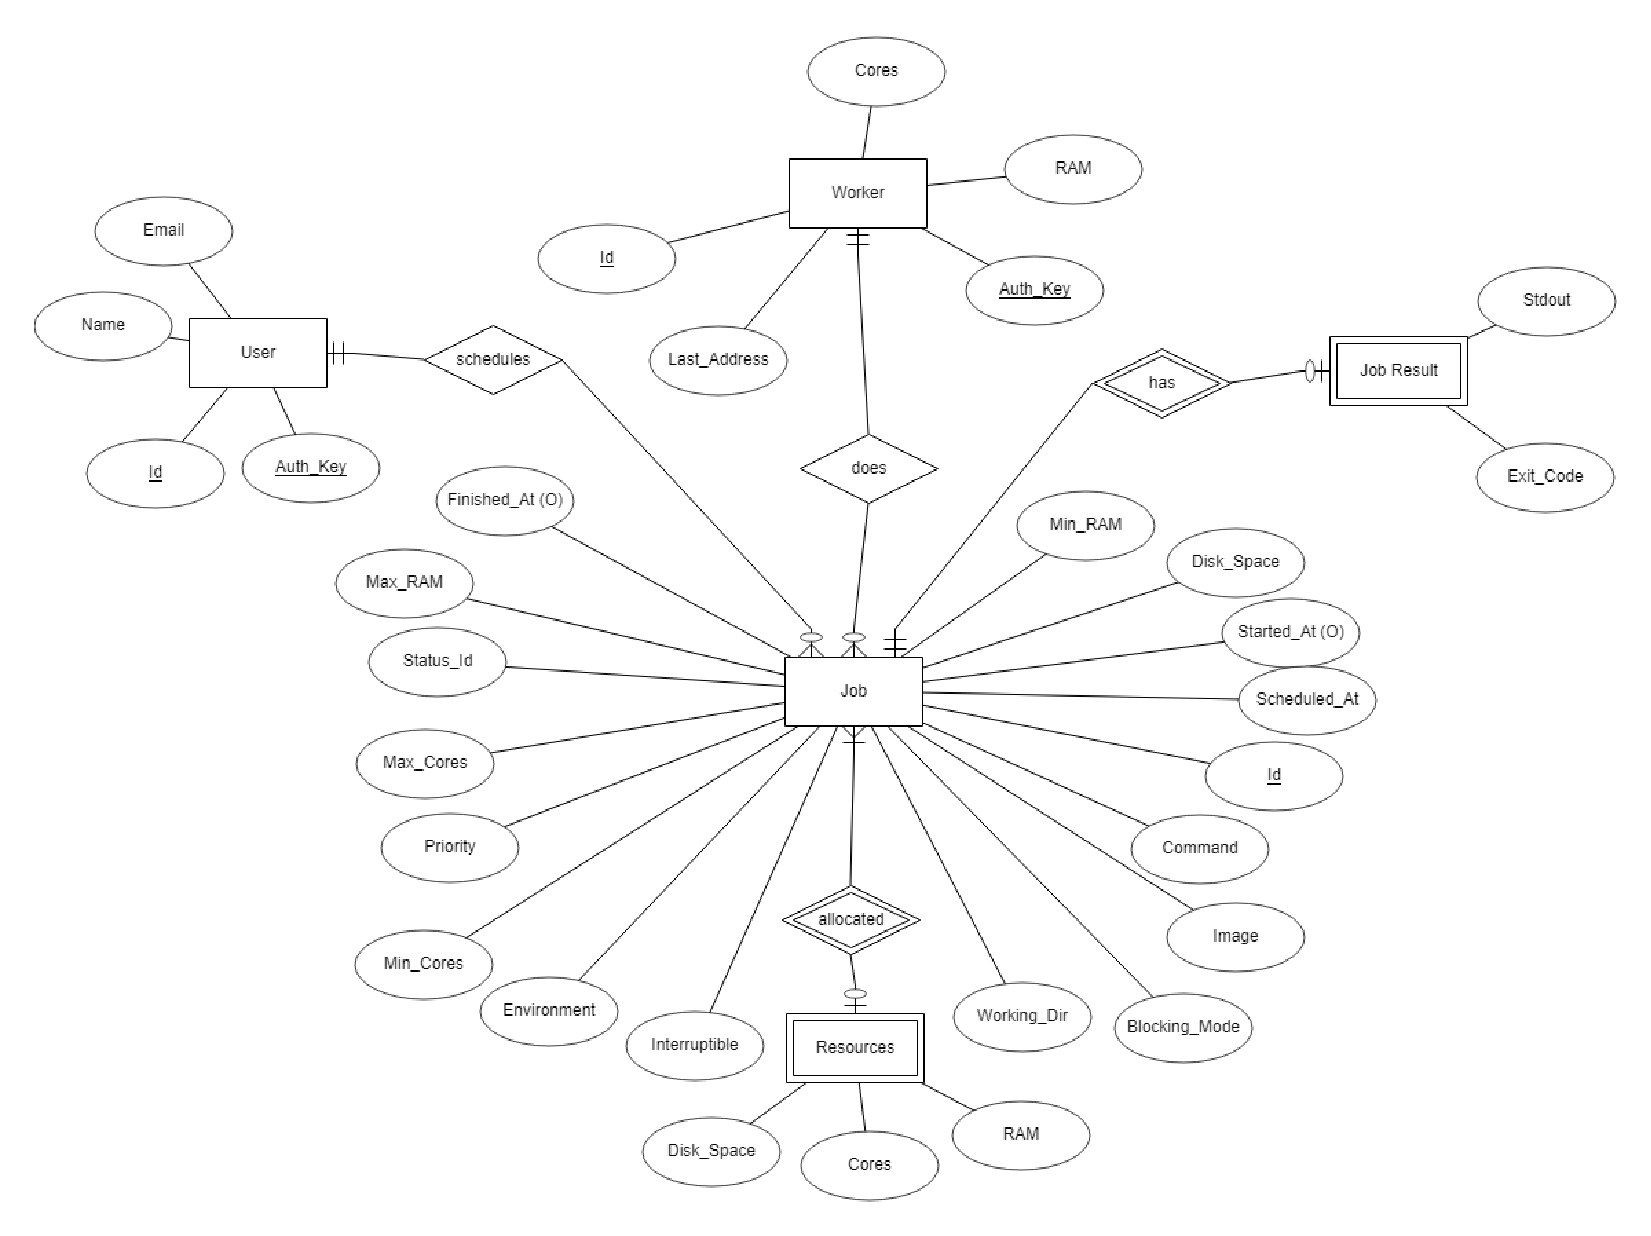
\includegraphics[width=\textwidth]{database_relational}

Die Datenbank ist in drei verschiedene Klassen unterteilt: Die Repository-, die Gateway- und die Factory-Klasse. Die Gateway-Klasse verwendet das Qt-Framework, um sich mit der Datenbank zu verbinden und die SQL-Queries durchzuführen. Die Factory-Klasse ist für die Erstellung von Objekten aus den vom Gateway zurückgegebenen Daten verantwortlich. Das Repository nutzt beide Klassen und dient als Schnittstelle für den Zugriff auf die Datenbank.


\subsection{Klassendiagramm}

% Übersicht aller Klassendiagramme




\clearpage
\section{Klassenbeschreibung}

\iffalse
Format:
\subsubsection{Klasse}

Kurze Beschreibung

\begin{itemize}[label={}]

	\item \textit{\textbf{Attribute}}
		\begin{itemize}[label={\textbullet}]
			\item \textit{name} beschreibung
		\end{itemize}

	\item \textit{\textbf{Methoden}}
		\begin{itemize}[label={\textbullet}]
			\item \textit{signatur} beschreibung
		\end{itemize}


\end{itemize}

\fi
\subsection{Datenbank}
\subsubsection{Model}
%Show the class diagram for it first



\subsubsection{Repository}

Die Repository-Klasse ist die Schnittstelle, die der Rest des Programms verwendet, um SQL-Queries durchzuführen und deren Ergebnisse zu interpretieren. Es verwendet die Gateway-Klasse, um die SQL-Queries durchzuführen und erzeugt ein Objekt, indem es der Factory-Klasse die von Gateway zurückgegebenen Daten gibt.

	\begin{itemize}[label={}]
	
		\item \textit{\textbf{Methoden}}
			\begin{itemize}[label={\textbullet}]
				\item \textit{public uint64\_t addWorker(int auth\_key, int space, int ram, int cores, std::string address)} Fügt einen Worker zur Datenbank hinzu und gibt seine ID zurück.
				
				\item \textit{public bool removeWorker(uint64\_t id)} Löscht einen Worker aus dem DB. Gibt true zurück, wenn die Operation erfolgreich war, ansonsten false.
				
				\item \textit{public Worker getWorker(uint64\_t worker\_id)} Gibt den Worker mit der angegebenen ID zurück.
				
				\item \textit{public std::vector<std::shared\_ptr<Worker>> getWorkers()} Gibt alle Workers zurück.
				
				\item \textit{public uint64\_t addJob(uint64\_t user\_id, JobConfig config, std::chrono::time\_point schedule\_time, std::string command)} Fügt einen Job zur Datenbank hinzu und gibt seine ID zurück. 
				
				\item \textit{public bool removeJob(uint64\_t job\_id)} Löscht einen Job aus dem DB. Gibt true zurück, wenn die Operation erfolgreich war, ansonsten false.
				
				\item \textit{public Job getJob(uint64\_t job\_id)} Gibt den Job mit der angegebenen ID zurück.
				
				\item \textit{public std::vector<std::shared\_ptr<Job>> getJobs()} Gibt alle Jobs zurück.
				
				\item \textit{public uint64\_t addUser(std::string name, std::string email, int auth\_key)} Fügt einen User zur Datenbank hinzu und gibt seine ID zurück. 
				
				\item \textit{public bool removeUser(uint64\_t user\_id)} Löscht einen User aus dem DB. Gibt true zurück, wenn die Operation erfolgreich war, ansonsten false.
				
				\item \textit{public User getUser(uint64\_t user\_id)} Gibt den User mit der angegebenen ID zurück.
				
				\item \textit{public std::vector<std::shared\_ptr<User>> getUsers()} Gibt alle Users zurück.
				
				\item \textit{public bool startJob(uint64\_t job\_id, uint64\_t worker\_id, specs specs, std::chrono::time\_point start\_time)} Aktualisiert den Eintrag eines Jobs in der Datenbank mit einer Startzeit, den zugewiesenen Ressourcen und dem zugeordneten Mitarbeiter. Gibt true zurück, wenn die Operation erfolgreich war, ansonsten false.
				
				\item \textit{public bool finishJob(uint64\_t job\_id, std::chrono::time\_point finish\_time, std::string stdout, int8\_t exit\_code)} Aktualisiert den Eintrag eines Jobs mit Endzeit, Ausgabe und Exitcode. Gibt true zurück, wenn die Operation erfolgreich war, ansonsten false.
				
				\item \textit{public job\_result getJobResult(uint64\_t job\_id)} Gibt die Ergebnisse eines \textbf{fertigen} Jobs zurück.
								
			\end{itemize}
			
	\end{itemize}
\subsubsection{Gateway}

Die Gateway-Klasse verbindet sich mit der Datenbank und führt die SQL-Queries aus.

\begin{itemize}[label={}]

	\item \textit{\textbf{Attribute}}
		\begin{itemize}[label={\textbullet}]
			\item \textit{QSqlDatabase db} Verwaltet die Verbindung zur Datenbank. 
		\end{itemize}

	\item \textit{\textbf{Methoden}}
		\begin{itemize}[label={\textbullet}]
			\item \textit{public uint64\_t addWorker(int auth\_key, int space, int ram, int cores, std::string address)} Fügt einen Worker zur Datenbank hinzu und gibt seine ID zurück.
				
				\item \textit{public bool removeWorker(int uint64\_t)} Löscht einen Worker aus dem DB. Gibt true zurück, wenn die Operation erfolgreich war, ansonsten false.
				
				\item \textit{public worker\_details getWorker(uint64\_t worker\_id)} Gibt die Daten des Workers mit der angegebenen ID zurück.
				
				\item \textit{public std::vector<std::shared\_ptr<worker\_details>> getWorkers()} Gibt die Daten jedes Mitarbeiters zurück.
				
				\item \textit{public uint64\_t addJob(uint64\_t user\_id, JobConfig config, std::chrono::time\_point schedule\_time, std::string command)} Fügt einen Job zur Datenbank hinzu und gibt seine ID zurück. 
				
				\item \textit{public bool removeJob(uint64\_t job\_id)} Löscht einen Job aus dem DB. Gibt true zurück, wenn die Operation erfolgreich war, ansonsten false.
				
				\item \textit{public job\_details getJob(uint64\_t job\_id)} Gibt die Daten des Jobs mit der angegebenen ID zurück.
				
				\item \textit{public std::vector<std::shared\_ptr<job\_details>> getJobs()} Gibt die Daten jedes Jobs zurück.
				
				\item \textit{public uint64\_t addUser(std::string name, std::string email, int auth\_key)} Fügt einen User zur Datenbank hinzu und gibt seine ID zurück. 
				
				\item \textit{public bool removeUser(uint64\_t user\_id)} Löscht einen User aus dem DB. Gibt true zurück, wenn die Operation erfolgreich war, ansonsten false.
				
				\item \textit{public user\_details getUser(uint64\_t user\_id)} Gibt die Daten des Users mit der angegebenen ID zurück
				
				\item \textit{public std::vector<std::shared\_ptr<user\_details>> getUsers()} Gibt die Daten jedes Users zurück.
				
				\item \textit{public bool startJob(uint64\_t job\_id, uint64\_t worker\_id, specs specs, std::chrono::time\_point start\_time)} Aktualisiert den Eintrag eines Jobs in der Datenbank mit einer Startzeit, den zugewiesenen Ressourcen und dem zugeordneten Mitarbeiter. Gibt true zurück, wenn die Operation erfolgreich war, ansonsten false.
				
				\item \textit{public bool finishJob(uint64\_t job\_id, std::chrono::time finish\_time, std::string stdout, int8\_t exit\_code)} Aktualisiert den Eintrag eines Jobs mit Endzeit, Ausgabe und Exitcode. Gibt true zurück, wenn die Operation erfolgreich war, ansonsten false.
				
				\item \textit{public job\_result getJobResult(uint64\_t job\_id)} Gibt die Ergebnisse eines \textbf{fertigen} Jobs zurück.
		\end{itemize}


\end{itemize}

\subsubsection{Factory}

Erzeugt Objekte aus gegebenen Daten.

\begin{itemize}[label={}]

	\item \textit{\textbf{Methoden}}
		\begin{itemize}[label={\textbullet}]
			\item \textit{public Job createJob(job\_details info)} Erzeugt ein Job-Objekt.
			
			\item \textit{public Worker createWorker(worker\_details info)} Erzeugt ein Worker-Objekt.
			
			\item \textit{public User createUser(user\_details info)} Erzeugt ein User-Objekt.
		\end{itemize}


\end{itemize}
\subsubsection{struct \purl{user_details}}

Eine struct, die alle relevanten Userdaten kapselt.

\begin{itemize}[label={}]

	\item \textit{\textbf{Attribute}}
		\begin{itemize}[label={\textbullet}]
			\item \textit{uint64\_t id} Eine eindeutige ID zur Identifizierung des Users.
			
			\item \textit{std::string name} Der Name des Users.
			
			\item \textit{std::string email} Die Email des Users.
			
			\item \textit{authkey} to be filled
		\end{itemize}


\end{itemize}

\subsubsection{struct specs}

Eine struct, die alle relevanten Hardware-Spezifikationen des Rechners kapselt.


\begin{itemize}[label={}]

	\item \textit{\textbf{Attribute}}
		\begin{itemize}[label={\textbullet}]
			\item \textit{int space} Speicherplatz.
			
			\item \textit{int ram} Random-Access Memory.
			
			\item \textit{int cores} Anzahl der CPU-Kerne.
			
		\end{itemize}


\end{itemize}

\subsubsection{struct \purl{worker_details}}

Eine struct, die alle relevanten Workerdaten kapselt.


\begin{itemize}[label={}]

	\item \textit{\textbf{Attribute}}
		\begin{itemize}[label={\textbullet}]
			\item \textit{uint64\_t id} Eine eindeutige ID zur Identifizierung des Workers.
			
			\item \textit{specs specs} Hardware-Spezifikationen des Rechners.
			
			\item \textit{std::string address}
			
			\item \textit{authkey} to be filled
		\end{itemize}


\end{itemize}
\clearpage

\subsubsection{struct \purl{job_details}}

Eine struct, die alle relevanten Jobdaten kapselt.

\begin{itemize}[label={}]

	\item \textit{\textbf{Attribute}}
		\begin{itemize}[label={\textbullet}]
			\item \textit{JobConfig config} Enthält die Konfiguration eines Jobs.
			
			\item \textit{uint64\_t user\_id} Die ID des Users, der diesen Job gescheduled hat.
			
			\item \textit{int status} Der Statuscode eines Jobs.
			
			\item \textit{uint64\_t id} Eine eindeutige ID zur Identifizierung des Jobs.
			
			\item \textit{std::string command} Der Befehl des Jobs, der in der Befehlszeile eingegeben wurde.
			
			\item \textit{std::chrono::time\_point schedule\_time} Die Uhrzeit, zu der der Job gescheduled wurde.
			
			\item \textit{std::chrono::time\_point start\_time} Die Uhrzeit, zu der der Job gestartet wurde.
			
			\item \textit{std::chrono::time\_point finish\_time} Die Uhrzeit, zu der der Job beendet wurde.
			
			\item \textit{specs allocated\_specs} Die Hardware-Ressourcen, die dem Job zugewiesen wurden.

		\end{itemize}


\end{itemize}


\subsubsection{CommandLineProcessor}

Der Command Line Processor (CLP) ist dafür zuständig, die Benutzereingabe auf der Befehlszeile in eine für das Programm verwendbare Struktur zu überführen. Es werden die Argumente auf der Befehlszeile eingelesen und mit vom Benutzer in einer Konfigurationsdatei angegebenen Standardwerten ergänzt. Anhand der Angaben auf der Befehlszeile kann erkannt werden, um welchen Typ von Befehl es sich handelt, und welche Parameter für die Ausführung des Befehls vorhanden sein müssen.

\begin{itemize}[label={}]

	\item \textit{\textbf{Attribute}}
		\begin{itemize}[label={\textbullet}]
		\end{itemize}

	\item \textit{\textbf{Methoden}}
		\begin{itemize}[label={\textbullet}]
			\item \textit{public Task process(char** argv, int* argc)} Verarbeitet Argumente der Befehlszeile.
			Weist jedem Argument zuerst den auf der Befehlszeile spezifizierten Wert, dann den vom Benutzer in einer Konfigurationsdatei hinterlegten Wert zu.
			Argumente, die nicht auf der Befehlszeile oder in der Konfigurationsdatei vorhanden sind, werden von dem Server mit Standardwerten verfollst�ndigt.\newline
			\newline
			argv: Array der Bezeichner sowie Werte der Argumente\newline
			argc: Anzahl der Eintr�ge in argv
			

			\item \textit{private void preProcess(char** argv, int* argc, std::shared_pointer<Task> task)}
			Baut aus den �bergebenen Argumenten einen Task auf.\newline
			Bestimmt den Typ der Anfrage (neue Aufgabe oder vorhandene Bearbeiten)\newline
			Hierbei werden komplexe Argumente von den eigentlichen Argumenten getrennt (z.B. wird der Aufgaben 	Startbefehl von den Argumenten unseres Programms abgetrennt, damit dies nicht zu Problemen in sp�teren
			Verarbeitungsschritten f�hrt).\newline
			argv und argc werden dementsprechend angepasst.\newline
			\newline
			argv: Array der Bezeichner und Werte der Argumente\newline
			argc: Anzahl der Eintr�ge in argv\newline
			task: Bekommt einen Aufgaben-Typ zugewiesen
			
			
			\item \textit{private void processArguments(char** argv, int* argc, std::shared_pointer<Task> task)}
			Wertet die Argumente der Befehlszeile aus und speichert sie in task.\newline
			Zusätzlich werden die Argumente aus der lokalen Konfigurationsdatei übernommen.\newline
			\newline
			argv: Array der Bezeichner und Werte der Argumente\newline
			argc: Anzahl der Eintr�ge in argv\newline
			task: Enthält nach Abarbeitungsende alle auf der Befehlszeile eingelesenen Argumente sowie alle Standardargumente der lokalen Konfigurationsdatei
			
			
		\end{itemize}


\end{itemize}

\clearpage

\subsubsection{Task}

Ein Task ist eine Repräsentation eines auf der Befehlszeile eingegebenen Befehls. Er enthält Informationen, die für die Ausführung des gewünschten Befehls wichtig sind. Dazu gehören im wesentlichen Befehlstyp sowie Argumente.

\begin{itemize}[label={}]

	\item \textit{\textbf{Attribute}}
		\begin{itemize}[label={\textbullet}]
			\item \textit{taskCommand} Startbefehl für die eingereichte Aufgabe
			\item \textit{config} Konfiguration dieses Befehls. Argumente der Befehlszeile und der lokalen Konfigurationsdatei.
			\item \textit{type} Gibt an, um was für eine Form von Anfrage es sich handelt (Starte neue Aufgabe oder frage etwas über eine existierende Aufgabe ab)
		\end{itemize}
		
	\item \textit{textbf{Methoden}}
		\begin{itemize}[label={\textbullet}]
		
			\item \textit{public int getType()} Gibt den Befehlstyp type zurück.
		
			\item \textit{public void setType(int type)} Setzt den Befehlstyp zu dem Angegebenen Typ. 
		
			\item \textit{public JobConfig getConfig()} Gibt Zugang zur Konfiguration des Befehls. Die Konfiguration kann von außerhalb beliebig modifiziert werden. 
		
			\item \textit{public std::string getTaskCommand()} Gibt den vom Benutzer spezifizierten Startbefehl der eingereichten Aufgabe (falls eine eingereicht wurde) so, wie er auf der Befehlszeile ausgeführt werden soll.
		
			\item \textit{public void setTaskCommand(const std::string\& taskCommand} Setzt den Startbefehl der eingereichten Aufgabe (falls eine eingereicht wurde).
		\end{itemize}

\end{itemize}


% Document ends here.
\printnoidxglossaries

\end{document}
